\subsection{Behavior} \label{requirementspecification:Behavior}

\subsubsection{Activity Diagram}
The Activity diagram, shown on Figure \ref{fig:actpackagepsosbehaviorprocess-overview}, shows how the different parts of the project work together. When the board has been started and software installed, the researcher is asked to configure the values $c1$ and $c2$, these are also known as the acceleration coefficients. $c1$ expresses how much confidence a particle has in itself, the cognitive aspect. $c2$ expresses how much confidence a particle has in its peers, the social aspect. A search for the minima can then be started and random values for the algorithm will be requested. When the random values has been obtained, the calculation occur and a result is returned.

\begin{figure}[H]
	\centering
	\includegraphics[width=0.7\linewidth]{"diagram/act_Package_PSOS_Behavior_Process Overview"}
	\caption{Activity diagram for PSOS}
	\label{fig:actpackagepsosbehaviorprocess-overview}
\end{figure}

\subsubsection{Sequence Diagram}
The sequence diagram in Figure \ref{fig:sdpsos}, shows the Sequence Diagram for the Zynq CPU.
It has a context, that is used to control the state pattern. Different actions and transitions are called.

\begin{figure}[H]
	\centering
	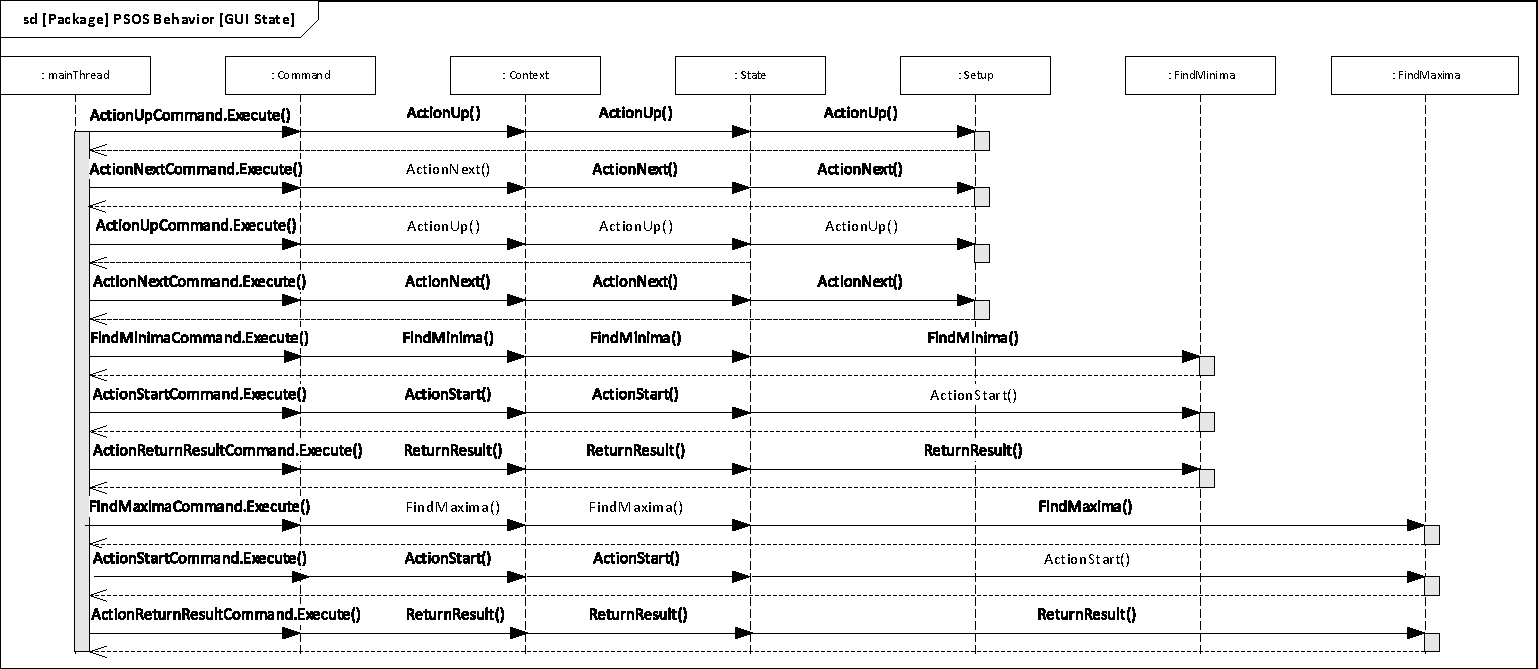
\includegraphics[width=1\linewidth]{diagram/sd_psos}
	\caption{Sequence Diagram for PSOS}
	\label{fig:sdpsos}
\end{figure}

\subsubsection{State Machine Diagram}\label{req:smd}

The State Machine in Figure \ref{fig:smdguistate} shows the different states that are allowed and how to traverse them. As can be observed, specific actions and transitions are allowed in the current state.

\begin{figure}[H]
	\centering
	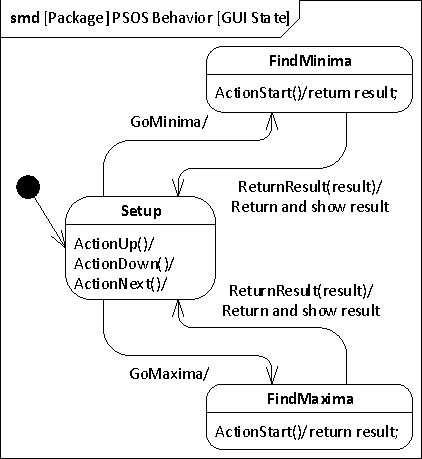
\includegraphics[width=0.4\linewidth]{diagram/smd_gui_state}
	\caption{State Machine Diagram of the Graphical User Interface}
	\label{fig:smdguistate}
\end{figure}
